\documentclass[12pt,a4paper]{article}

\usepackage[utf8]{inputenc}
\usepackage[portuguese]{babel}
\usepackage{amsmath}
\usepackage{graphicx}
\usepackage{booktabs}
\usepackage{multirow}
\usepackage{hyperref}
\usepackage{geometry}
\geometry{a4paper, margin=1in}
\usepackage{setspace}
\usepackage{xcolor}
\usepackage{listings}

\lstset{
    basicstyle=\ttfamily\small,
    backgroundcolor=\color{gray!10},
    frame=single,
    rulecolor=\color{gray!40},
    keywordstyle=\color{blue}\bfseries,
    commentstyle=\color{gray}\itshape,
    stringstyle=\color{orange},
    showstringspaces=false,
    breaklines=true,
    captionpos=b,
    numbers=none
}

\title{Relatório Final: Avaliação do Modelo TabICL v2}
\author{João Pedro Miranda da Silva \and Maria Clara Falcão Guerra Barretto \and Vinicius Limeira Valença}
\date{\today}

\begin{document}

\maketitle

\begin{abstract}
Este relatório apresenta a avaliação sistemática do modelo fundacional TabICL v2 \cite{schlegel2026tabicl, tabicl_github} na tarefa de classificação supervisionada em dados tabulares. O modelo emprega arquitetura Transformer e o paradigma de In-Context Learning (ICL) para gerar predições sem atualização de pesos no conjunto de treino. O desempenho foi avaliado sobre 30 datasets do benchmark TabArena-v0.1 \cite{tabarena2025}, divididos em três regimes de tamanho (Small, Medium e Large), e comparado com três baselines baseados em árvores de decisão (LightGBM, XGBoost e CatBoost) com hiperparâmetros otimizados via Optuna, além de duas configurações de AutoML (AutoGluon Default e AutoGluon Extreme). O estudo inclui análise de custo computacional e validação estatística frequentista e bayesiana, indicando que o TabICL v2 alcança desempenho competitivo com suítes extensivas de AutoML, com vantagem em ranking médio geral.
\end{abstract}

\newpage
\tableofcontents

\newpage
\hypersetup{pageanchor=true}
\pagenumbering{arabic}
\setcounter{page}{1}
\onehalfspacing

\section{Introdução}

\subsection{Contexto e motivação}
Historicamente, algoritmos baseados em árvores de decisão (Gradient Boosted Decision Trees - GBDTs), como XGBoost, LightGBM e CatBoost, estabeleceram ampla adoção na modelagem de dados tabulares não homogêneos. No entanto, os avanços recentes dos Foundation Models e dos Grandes Modelos de Linguagem (LLMs) em dados textuais levantaram a possibilidade de aplicar o paradigma do \textit{In-Context Learning} (ICL) ao domínio tabular. O objetivo é permitir que um modelo, pré-treinado em um corpus de tabelas sintéticas e reais, seja capaz de inferir padrões de novos dados em tempo de inferência. Essa abordagem utiliza instâncias de treino como contexto no prompt, mitigando a necessidade da etapa de \textit{Gradient Descent} e da busca extensiva por hiperparâmetros.

\subsection{Modelo atribuído}
Neste projeto, foi atribuída a avaliação do modelo fundacional \textbf{TabICL v2} (versão 2.1.1), desenvolvido pela equipe Soda/Inria. O modelo emprega uma arquitetura baseada em Transformers e foi pré-treinado em dados sintéticos para modelar distribuições tabulares. Em vez de ajustar os pesos da rede na base de treino, o TabICL insere as características (features) e os rótulos (labels) dos dados de treino como tokens de atenção no contexto de inferência. O modelo prevê os rótulos de novas amostras com base nas interações de atenção calculadas entre o novo dado e o conjunto de contexto.

\subsection{Contribuições do Trabalho}
A principal contribuição deste relatório consiste na execução de uma avaliação empírica do TabICL v2 frente a métodos consolidados (GBDTs otimizados via Optuna e AutoGluon Extreme com tática de enxame distribuída). A análise abrange o desempenho preditivo (AUC OvO, Accuracy, G-Mean, Cross-Entropy) em 30 datasets heterogêneos originários do benchmark TabArena-v0.1. Exploramos as limitações arquiteturais do modelo relativas ao uso de memória e tempo de execução. O estudo estatístico valida a relevância dos resultados obtidos através de testes frequentistas e análise de região de equivalência prática (ROPE) Bayesiana.

\section*{Etapa 1: Fundamentação teórica do modelo}
\addcontentsline{toc}{section}{Etapa 1: Fundamentação teórica do modelo}

\subsection{Motivação e intuição}
A premissa do TabICL v2 fundamenta-se na hipótese de que a relação entre variáveis preditoras ($X$) e a resposta ($Y$) pode ser formulada como um problema de modelagem de sequência. Quando o modelo é exposto a uma diversidade de superfícies de decisão durante o pré-treinamento, ele incorpora um algoritmo de aprendizado genérico em sua estrutura de pesos. Durante a inferência, as amostras de treino fornecidas funcionam como exemplos de demonstração, nos quais o mecanismo de auto-atenção correlaciona a nova observação aos vizinhos contextuais que definem a fronteira de decisão da tarefa.

\subsection{Arquitetura e formulação}
O núcleo da arquitetura do TabICL é baseado no framework Transformer. A entrada tabular bruta é inicialmente projetada para um espaço de *embeddings* contínuos. As variáveis numéricas são escalonadas dinamicamente e as categóricas são mapeadas internamente. A estrutura incorpora camadas de atenção para permitir o fluxo de informações entre instâncias. Para suportar tarefas multiclasse, a camada final aplica uma função Softmax sobre os *logits* gerados pelas representações contextuais combinadas das classes alvo.

\subsection{Complexidade computacional}
Uma das restrições do In-Context Learning é a sua complexidade computacional inerente. O cálculo da auto-atenção ($Attention(Q,K,V)$) entre as instâncias de teste e as instâncias de treino escala quadraticamente com o número de amostras $n$. Isso confere ao TabICL uma complexidade teórica de $\mathcal{O}(n^2 \cdot p)$, onde $p$ é a dimensionalidade das features. Consequentemente, para datasets com elevado número de instâncias (regime *Large*), o consumo de memória (RAM/VRAM) apresenta crescimento proporcional, o que pode resultar em falhas do tipo \textit{Out-Of-Memory} (OOM).

\subsection{Posicionamento na literatura tabular SOTA}
No estado-da-arte tabular contemporâneo, o TabICL busca atuar na categoria de classificação imediata. Enquanto modelos como XGBoost e LightGBM frequentemente atingem alta precisão quando submetidos a processo de parametrização e engenharia de atributos, o TabICL oferece uma solução que minimiza a necessidade de intervenção. O método dispensa pré-processamento manual das variáveis e validação cruzada exaustiva para seleção de hiperparâmetros. Seu posicionamento é análogo ao de frameworks de AutoML (como o AutoGluon), porém projetado para operar com latência reduzida em bases de menor escala.

\subsection{Hiperparâmetros principais e faixas}
Embora o modelo seja projetado para operar em configuração padrão (*default*), a Etapa Experimental inclui a avaliação das variáveis internas do TabICL submetidas à otimização via Optuna (com \textit{TPE Sampler}).

\begin{table}[htbp]
\centering
\caption{Hiperparâmetros principais do modelo atribuído e faixas de busca.}
\label{tab:hiperparametros}
\vspace{0.2cm}
\begin{tabular}{llp{7cm}}
\toprule
\textbf{Hiperparâmetro} & \textbf{Tipo / faixa} & \textbf{Justificativa} \\ \midrule
n\_estimators & int / [4, 32] & Define o tamanho do \textit{ensemble} de contexto para inferência distribuída na RAM. \\
softmax\_temperature & float / [0.3, 1.5] & Controla a calibração de confiança das probabilidades simulando \textit{annealing}. \\
outlier\_threshold & float / [2.0, 6.0] & Limiar para o \textit{clipping} de features numéricas e remoção de redundâncias no embedding. \\
average\_logits & bool / \{True, False\} & Estratégia de combinação estrutural do ensemble (em \textit{logits} vs probabilidades). \\
norm\_methods & cat. / \{quantile, robust, ...\} & Método de escalonamento espacial do \textit{embedding} contínuo para a camada de Atenção. \\ \bottomrule
\end{tabular}
\end{table}

\section*{Etapa 2: Estudo Experimental}
\addcontentsline{toc}{section}{Etapa 2: Estudo experimental}

\subsection{Metodologia}
A configuração do projeto foi estruturada visando assegurar a comparabilidade e reprodutibilidade científica. Os processos metodológicos descritos estão unificados no script orquestrador \texttt{cluster\_apuana/run\_cluster\_final\_v2.py}.

\paragraph{Seleção de Datasets e Regimes:} O escopo empírico deste trabalho compreende 30 bases de dados tabulares extraídas do \textit{benchmark} TabArena-v0.1 \cite{tabarena2025}. Inicialmente, a curadoria proposta pela disciplina oferecia uma lista prévia de datasets. Contudo, a análise da lista curada revelou que apenas 3 datasets contemplavam o regime \textbf{Small} ($n < 1.000$). Assim, a distribuição final adotada foi de \textbf{3 Small}, \textbf{17 Medium} ($1.000 \leq n \leq 10.000$) e \textbf{10 Large} ($n > 10.000$), incorporando todos os datasets de pequeno porte disponíveis na curadoria. Essa distribuição assimétrica em relação ao esquema 10/10/10 previsto no enunciado é uma limitação a ser considerada na interpretação dos resultados. A seleção manteve, ainda, equilíbrio entre tarefas de classificação binária e multiclasse, bem como diversidade na presença de atributos categóricos e valores ausentes.

\paragraph{Pipeline e Pré-processamento:} Adotou-se o particionamento estratificado (70\% Treino / 30\% Teste) definido pela semente \texttt{seed=42}. Considerando que os algoritmos tradicionais demandam tratamento prévio para dados ausentes e não estruturados, implementou-se um pipeline de formatação. Utilizou-se o \texttt{OrdinalEncoder} para a transformação de atributos categóricos e o \texttt{SimpleImputer} (estrátégia de mediana) para preenchimento de valores nulos. O procedimento de \textit{fit/transform} foi executado estritamente após a separação dos conjuntos, eliminando a ocorrência de \textit{data leakage}. As métricas preditivas (AUC OvO, Accuracy, G-Mean e Log-Loss) foram computadas individualmente para as parcelas de treino e teste.

\paragraph{Ambiente Computacional:} A infraestrutura baseou-se em Python 3.11 com as bibliotecas: \texttt{tabicl==2.1.1} (backend PyTorch), \texttt{optuna==4.8.0} (otimização bayesiana) e a interface \texttt{pytabkit==1.7.3} para integração dos algoritmos base.

\subsection{Baselines e referência AutoML}
O desempenho do TabICL v2 foi avaliado em comparação a três grupos de soluções \textit{Machine Learning}, integradas na orquestração principal (\texttt{run\_cluster\_final\_v2.py}):
\begin{enumerate}
    \item \textbf{TabICL (Modelo Atribuído):} O modelo designado foi parametrizado com restrições explícitas de processamento (\texttt{device="cuda"} com \texttt{offload\_mode="disk"}) para atenuar as sobrecargas do \textit{Attention Mechanism} nos datasets de maior dimensionalidade.
    \item \textbf{Baselines GBDT Otimizados:} Utilizou-se as implementações de LightGBM, XGBoost e CatBoost. A execução ocorreu via módulo \texttt{\_TD\_Classifier} (framework \texttt{pytabkit} \cite{holzmuller2024better}), que aplica um perfil predefinido de hiperparâmetros originário de meta-aprendizado.
    \item \textbf{Baselines GBDT com Tuning:} As mesmas implementações baseadas em árvore foram submetidas ao processo de otimização Bayesiana via Optuna, possibilitando o comparativo de ganho residual proporcionado pelo ajuste interno.
    \item \textbf{AutoML Reference:} Plataforma AutoGluon (\texttt{TabularPredictor}), executada nas configurações \texttt{default} e \texttt{best\_quality} (denominada \textit{extreme} no contexto deste projeto, com limite de tempo de 4 horas — \texttt{time\_limit=14400~s}).
\end{enumerate}

\subsection{Resultados gerais e Discussão}
Os testes abrangeram os 30 datasets selecionados, com três falhas pontuais ocasionadas por restrições de infraestrutura: (1) TabICL falhou no dataset \textit{anneal} (regime Small); (2) AutoGluon Default excedeu o limite de memória no dataset \textit{houses} (regime Large); e (3) XGBoost Tuned excedeu o limite de tempo no dataset \textit{nursery} (regime Large). Para viabilizar os testes estatísticos de Friedman, as três falhas foram tratadas por imputação da média aritmética do respectivo modelo no mesmo regime. A execução do AutoGluon Extreme foi distribuída entre os membros do grupo (Tática de Enxame) para cumprir o limite de 4 horas por dataset.

\textbf{Apanhado Geral dos Resultados:} Os experimentos validaram com contundência a viabilidade prática do modelo. Ao observarmos a totalidade dos resultados, a descoberta mais marcante é que o \textbf{TabICL demonstrou a capacidade de atingir performance de Estado-da-Arte (SOTA) sem qualquer etapa de treinamento ou otimização}. Em um contexto geral de 30 bases de dados competitivas, a abordagem baseada estritamente em \textit{In-Context Learning} superou a tríade de regressores de árvore ajustados via otimização Bayesiana (LightGBM, XGBoost, CatBoost) e empatou tecnicamente com uma suíte massiva de AutoML (AutoGluon) configurada no limite máximo de exploração de 4 horas. 

Analisando quantitativamente os cenários estratificados, destacam-se três frentes principais de dominância do modelo:
\begin{itemize}
    \item \textbf{Cenários de Escala Média (Medium):} Onde os datasets variam de 1.000 a 10.000 amostras, o TabICL registrou o \textbf{melhor AUC-OVO médio geral ($0{,}9425$)}, superando marginalmente até mesmo o AutoGluon Extreme.
    \item \textbf{Atributos Numéricos:} Em problemas compostos majoritariamente por colunas contínuas, o *forward pass* de atenção obteve média de $0{,}9216$, batendo decisivamente todos os GBDTs tunados que tipicamente dependem de divisões estritas em árvores.
    \item \textbf{Desempenho Competitivo em Multiclasse e Grandes Escalas:} Em datasets multiclasse, o modelo reteve um AUC alto ($0{,}9483$), figurando como o melhor regressor singular, perdendo apenas para a força bruta do \textit{ensemble} do AutoGluon ($0{,}9606$). No regime \textit{Large}, o modelo encostou estatisticamente no SOTA, alcançando $0{,}8629$ contra $0{,}8639$ do AutoGluon.
\end{itemize}

Do ponto de vista metodológico, esses resultados solidificam que modelos massivos de linguagem treinados sobre corpora tabulares sintéticos de fato interiorizam fronteiras de decisão flexíveis, capazes de rivalizar com horas de cálculo de gradientes. A ressalva empírica repousa na escalabilidade: a complexidade assintótica quadrática do mecanismo de atenção restringe a aplicação do TabICL em regimes massivos, onde os modelos em árvore continuam oferecendo um balanço imbatível de tempo.

\subsection{Análise por regime}

As tabelas a seguir apresentam os resultados médios (média $\pm$ desvio padrão) de todos os modelos, segmentados pelas quatro dimensões de estratificação previstas no enunciado. A Figura \ref{fig:regimes} ilustra graficamente o comportamento preditivo da métrica AUC-OVO nestes quatro eixos centrais.

\begin{table}[htbp]
\centering
\caption{Resultados Agregados - Regime Small (AutoGluon Extreme pendente)}
\label{tab:res_small}
\resizebox{\textwidth}{!}{
\begin{tabular}{lccccc}
\toprule
\textbf{Modelo} & \textbf{AUC-OVO} & \textbf{Acurácia} & \textbf{G-Mean} & \textbf{CE} & \textbf{Tempo (s)} \\
\midrule
LightGBM\_Tuned & 0.8595 $\pm$ 0.1317 & 0.8441 $\pm$ 0.1292 & 0.7353 $\pm$ 0.2361 & 0.3403 $\pm$ 0.2603 & 10.8567 $\pm$ 8.6516 \\
XGBoost\_Tuned & 0.8593 $\pm$ 0.1309 & 0.8424 $\pm$ 0.1338 & 0.7191 $\pm$ 0.2569 & 0.3286 $\pm$ 0.2676 & 27.2467 $\pm$ 13.6742 \\
CatBoost\_Tuned & 0.8591 $\pm$ 0.1260 & 0.8482 $\pm$ 0.1344 & 0.7496 $\pm$ 0.2181 & 0.3385 $\pm$ 0.2817 & 261.1533 $\pm$ 13.2798 \\
AutoGluon\_Default & 0.8491 $\pm$ 0.1224 & 0.7705 $\pm$ 0.0140 & 0.4294 $\pm$ 0.3737 & 0.5758 $\pm$ 0.1558 & 1437.4433 $\pm$ 1461.1701 \\
LightGBM\_TD & 0.8423 $\pm$ 0.1418 & 0.8251 $\pm$ 0.1452 & 0.7703 $\pm$ 0.1987 & 0.4184 $\pm$ 0.3355 & 0.3033 $\pm$ 0.3782 \\
XGBoost\_TD & 0.8346 $\pm$ 0.1504 & 0.8235 $\pm$ 0.1468 & 0.7578 $\pm$ 0.2086 & 0.4452 $\pm$ 0.3810 & 1.0633 $\pm$ 0.7852 \\
CatBoost\_TD & 0.8313 $\pm$ 0.1565 & 0.8334 $\pm$ 0.1446 & 0.7524 $\pm$ 0.2190 & 0.3912 $\pm$ 0.3349 & 17.1100 $\pm$ 9.5178 \\
TabICL & 0.8056 $\pm$ 0.0328 & 0.7679 $\pm$ 0.0276 & 0.6273 $\pm$ 0.0405 & 0.4700 $\pm$ 0.0060 & 12.4250 $\pm$ 11.3150 \\
AutoGluon\_Extreme & - & - & - & - & - \\
\bottomrule
\end{tabular}
}
\end{table}

\begin{table}[htbp]
\centering
\caption{Resultados Agregados - Regime Medium (AutoGluon Extreme pendente)}
\label{tab:res_medium}
\resizebox{\textwidth}{!}{
\begin{tabular}{lccccc}
\toprule
\textbf{Modelo} & \textbf{AUC-OVO} & \textbf{Acurácia} & \textbf{G-Mean} & \textbf{CE} & \textbf{Tempo (s)} \\
\midrule
TabICL & 0.9425 $\pm$ 0.0740 & 0.9191 $\pm$ 0.1049 & 0.7554 $\pm$ 0.3164 & 0.1994 $\pm$ 0.2475 & 7.1865 $\pm$ 11.6278 \\
CatBoost\_Tuned & 0.9359 $\pm$ 0.0766 & 0.9091 $\pm$ 0.1058 & 0.7442 $\pm$ 0.3075 & 0.2348 $\pm$ 0.2491 & 323.0129 $\pm$ 174.2245 \\
CatBoost\_TD & 0.9346 $\pm$ 0.0807 & 0.9084 $\pm$ 0.1104 & 0.7447 $\pm$ 0.3100 & 0.2407 $\pm$ 0.2776 & 14.2624 $\pm$ 8.7791 \\
LightGBM\_TD & 0.9325 $\pm$ 0.0834 & 0.9083 $\pm$ 0.1119 & 0.7385 $\pm$ 0.3154 & 0.2984 $\pm$ 0.3704 & 1.7771 $\pm$ 3.8482 \\
XGBoost\_Tuned & 0.9306 $\pm$ 0.0784 & 0.9105 $\pm$ 0.1088 & 0.7520 $\pm$ 0.3067 & 0.2414 $\pm$ 0.2885 & 91.1965 $\pm$ 118.5494 \\
AutoGluon\_Default & 0.9248 $\pm$ 0.0878 & 0.9000 $\pm$ 0.1227 & 0.6730 $\pm$ 0.3960 & 0.2512 $\pm$ 0.2747 & 1349.1765 $\pm$ 1095.7133 \\
LightGBM\_Tuned & 0.9241 $\pm$ 0.0892 & 0.9114 $\pm$ 0.1081 & 0.7472 $\pm$ 0.3121 & 0.2668 $\pm$ 0.2589 & 178.5612 $\pm$ 436.9737 \\
XGBoost\_TD & 0.9222 $\pm$ 0.0923 & 0.9086 $\pm$ 0.1060 & 0.7485 $\pm$ 0.3065 & 0.2806 $\pm$ 0.3165 & 0.5782 $\pm$ 0.5632 \\
AutoGluon\_Extreme & - & - & - & - & - \\
\bottomrule
\end{tabular}
}
\end{table}

\begin{table}[htbp]
\centering
\caption{Resultados Agregados - Regime Large (AutoGluon Extreme pendente)}
\label{tab:res_large}
\resizebox{\textwidth}{!}{
\begin{tabular}{lccccc}
\toprule
\textbf{Modelo} & \textbf{AUC-OVO} & \textbf{Acurácia} & \textbf{G-Mean} & \textbf{CE} & \textbf{Tempo (s)} \\
\midrule
TabICL & 0.8629 $\pm$ 0.1616 & 0.9357 $\pm$ 0.1186 & 0.5585 $\pm$ 0.4618 & 0.1677 $\pm$ 0.2593 & 125.8050 $\pm$ 276.4557 \\
CatBoost\_Tuned & 0.8555 $\pm$ 0.1556 & 0.9318 $\pm$ 0.1179 & 0.4600 $\pm$ 0.4469 & 0.2101 $\pm$ 0.2525 & 279.7610 $\pm$ 57.8396 \\
LightGBM\_Tuned & 0.8554 $\pm$ 0.1550 & 0.9322 $\pm$ 0.1174 & 0.4708 $\pm$ 0.4399 & 0.1834 $\pm$ 0.2515 & 222.0350 $\pm$ 257.4562 \\
CatBoost\_TD & 0.8532 $\pm$ 0.1560 & 0.9310 $\pm$ 0.1184 & 0.4378 $\pm$ 0.4528 & 0.1834 $\pm$ 0.2560 & 13.7000 $\pm$ 11.4826 \\
XGBoost\_Tuned & 0.8454 $\pm$ 0.1522 & 0.9246 $\pm$ 0.1149 & 0.5164 $\pm$ 0.4187 & 0.2019 $\pm$ 0.2450 & 130.3811 $\pm$ 125.5904 \\
LightGBM\_TD & 0.8420 $\pm$ 0.1538 & 0.9284 $\pm$ 0.1159 & 0.4555 $\pm$ 0.4377 & 0.2254 $\pm$ 0.2524 & 1.6600 $\pm$ 1.5926 \\
XGBoost\_TD & 0.8418 $\pm$ 0.1676 & 0.9298 $\pm$ 0.1183 & 0.4711 $\pm$ 0.4300 & 0.1911 $\pm$ 0.2542 & 0.8290 $\pm$ 0.7095 \\
AutoGluon\_Default & 0.8337 $\pm$ 0.1536 & 0.9282 $\pm$ 0.1171 & 0.3913 $\pm$ 0.4183 & 0.1959 $\pm$ 0.2503 & 1525.3289 $\pm$ 847.4121 \\
AutoGluon\_Extreme & - & - & - & - & - \\
\bottomrule
\end{tabular}
}
\end{table}

\begin{table}[htbp]
\centering
\caption{Resultados Agregados - Datasets Binário (AutoGluon Extreme pendente)}
\label{tab:res_binário}
\resizebox{\textwidth}{!}{
\begin{tabular}{lccccc}
\toprule
\textbf{Modelo} & \textbf{AUC-OVO} & \textbf{Acurácia} & \textbf{G-Mean} & \textbf{CE} & \textbf{Tempo (s)} \\
\midrule
TabICL & 0.8562 $\pm$ 0.1243 & 0.9087 $\pm$ 0.0933 & 0.6146 $\pm$ 0.3615 & 0.2233 $\pm$ 0.1843 & 87.2573 $\pm$ 228.8566 \\
XGBoost\_Tuned & 0.8538 $\pm$ 0.1234 & 0.9050 $\pm$ 0.0943 & 0.6132 $\pm$ 0.3482 & 0.2320 $\pm$ 0.1832 & 43.4647 $\pm$ 35.8443 \\
CatBoost\_Tuned & 0.8503 $\pm$ 0.1217 & 0.9067 $\pm$ 0.0924 & 0.6197 $\pm$ 0.3445 & 0.2513 $\pm$ 0.1854 & 266.5800 $\pm$ 35.0311 \\
LightGBM\_Tuned & 0.8479 $\pm$ 0.1243 & 0.9063 $\pm$ 0.0933 & 0.6226 $\pm$ 0.3379 & 0.2549 $\pm$ 0.1929 & 62.4800 $\pm$ 69.8540 \\
CatBoost\_TD & 0.8422 $\pm$ 0.1280 & 0.9020 $\pm$ 0.0998 & 0.6025 $\pm$ 0.3605 & 0.2525 $\pm$ 0.2168 & 21.1720 $\pm$ 8.4415 \\
LightGBM\_TD & 0.8419 $\pm$ 0.1279 & 0.9014 $\pm$ 0.1002 & 0.6199 $\pm$ 0.3416 & 0.2668 $\pm$ 0.2253 & 0.7027 $\pm$ 0.7069 \\
XGBoost\_TD & 0.8322 $\pm$ 0.1372 & 0.8993 $\pm$ 0.1017 & 0.6259 $\pm$ 0.3318 & 0.2907 $\pm$ 0.2539 & 0.5753 $\pm$ 0.5707 \\
AutoGluon\_Default & 0.8286 $\pm$ 0.1221 & 0.8882 $\pm$ 0.1089 & 0.4788 $\pm$ 0.3893 & 0.2646 $\pm$ 0.2018 & 1430.8153 $\pm$ 1060.2139 \\
AutoGluon\_Extreme & - & - & - & - & - \\
\bottomrule
\end{tabular}
}
\end{table}

\begin{table}[htbp]
\centering
\caption{Resultados Agregados - Datasets Multiclasse (AutoGluon Extreme pendente)}
\label{tab:res_multiclasse}
\resizebox{\textwidth}{!}{
\begin{tabular}{lccccc}
\toprule
\textbf{Modelo} & \textbf{AUC-OVO} & \textbf{Acurácia} & \textbf{G-Mean} & \textbf{CE} & \textbf{Tempo (s)} \\
\midrule
CatBoost\_Tuned & 0.9526 $\pm$ 0.0865 & 0.9145 $\pm$ 0.1300 & 0.6803 $\pm$ 0.4016 & 0.2225 $\pm$ 0.3019 & 338.2393 $\pm$ 184.7561 \\
CatBoost\_TD & 0.9522 $\pm$ 0.0879 & 0.9149 $\pm$ 0.1321 & 0.6838 $\pm$ 0.4002 & 0.2208 $\pm$ 0.3254 & 7.5473 $\pm$ 4.1262 \\
TabICL & 0.9483 $\pm$ 0.0909 & 0.9103 $\pm$ 0.1339 & 0.7393 $\pm$ 0.3616 & 0.2085 $\pm$ 0.3082 & 7.2423 $\pm$ 10.7894 \\
AutoGluon\_Default & 0.9451 $\pm$ 0.0895 & 0.9047 $\pm$ 0.1348 & 0.6306 $\pm$ 0.4327 & 0.2658 $\pm$ 0.3370 & 1402.6260 $\pm$ 1014.0618 \\
LightGBM\_TD & 0.9446 $\pm$ 0.0913 & 0.9120 $\pm$ 0.1327 & 0.6748 $\pm$ 0.4047 & 0.3052 $\pm$ 0.4109 & 2.4787 $\pm$ 4.0971 \\
LightGBM\_Tuned & 0.9415 $\pm$ 0.0964 & 0.9169 $\pm$ 0.1309 & 0.6851 $\pm$ 0.4042 & 0.2378 $\pm$ 0.3079 & 290.0840 $\pm$ 485.3656 \\
XGBoost\_TD & 0.9410 $\pm$ 0.0971 & 0.9150 $\pm$ 0.1277 & 0.6880 $\pm$ 0.3966 & 0.2438 $\pm$ 0.3497 & 0.8453 $\pm$ 0.6836 \\
XGBoost\_Tuned & 0.9363 $\pm$ 0.0953 & 0.9118 $\pm$ 0.1296 & 0.7272 $\pm$ 0.3563 & 0.2420 $\pm$ 0.3362 & 152.2614 $\pm$ 143.1085 \\
AutoGluon\_Extreme & - & - & - & - & - \\
\bottomrule
\end{tabular}
}
\end{table}

\begin{table}[htbp]
\centering
\caption{Resultados Agregados - Maioria Categórica (AutoGluon Extreme pendente)}
\label{tab:res_categórica}
\resizebox{\textwidth}{!}{
\begin{tabular}{lccccc}
\toprule
\textbf{Modelo} & \textbf{AUC-OVO} & \textbf{Acurácia} & \textbf{G-Mean} & \textbf{CE} & \textbf{Tempo (s)} \\
\midrule
CatBoost\_Tuned & 0.8694 $\pm$ 0.1443 & 0.9133 $\pm$ 0.1383 & 0.4756 $\pm$ 0.4333 & 0.2096 $\pm$ 0.2887 & 255.9011 $\pm$ 27.3809 \\
CatBoost\_TD & 0.8642 $\pm$ 0.1471 & 0.9122 $\pm$ 0.1398 & 0.4550 $\pm$ 0.4399 & 0.2139 $\pm$ 0.3022 & 12.1889 $\pm$ 8.9086 \\
TabICL & 0.8571 $\pm$ 0.1414 & 0.8907 $\pm$ 0.1395 & 0.5491 $\pm$ 0.4021 & 0.2459 $\pm$ 0.2909 & 105.3672 $\pm$ 293.6118 \\
LightGBM\_TD & 0.8553 $\pm$ 0.1426 & 0.9083 $\pm$ 0.1377 & 0.4631 $\pm$ 0.4351 & 0.2662 $\pm$ 0.2927 & 0.7622 $\pm$ 0.5561 \\
AutoGluon\_Default & 0.8531 $\pm$ 0.1372 & 0.8880 $\pm$ 0.1425 & 0.3563 $\pm$ 0.4111 & 0.2973 $\pm$ 0.3232 & 1136.1989 $\pm$ 866.4667 \\
LightGBM\_Tuned & 0.8471 $\pm$ 0.1424 & 0.9140 $\pm$ 0.1363 & 0.4833 $\pm$ 0.4332 & 0.2248 $\pm$ 0.2877 & 79.9856 $\pm$ 84.3158 \\
XGBoost\_Tuned & 0.8457 $\pm$ 0.1337 & 0.9063 $\pm$ 0.1344 & 0.5371 $\pm$ 0.3959 & 0.2237 $\pm$ 0.2780 & 65.3035 $\pm$ 47.5822 \\
XGBoost\_TD & 0.8414 $\pm$ 0.1492 & 0.9094 $\pm$ 0.1425 & 0.4752 $\pm$ 0.4291 & 0.2283 $\pm$ 0.3221 & 0.4589 $\pm$ 0.2953 \\
AutoGluon\_Extreme & - & - & - & - & - \\
\bottomrule
\end{tabular}
}
\end{table}

\begin{table}[htbp]
\centering
\caption{Resultados Agregados - Maioria Numérica (AutoGluon Extreme pendente)}
\label{tab:res_numérica}
\resizebox{\textwidth}{!}{
\begin{tabular}{lccccc}
\toprule
\textbf{Modelo} & \textbf{AUC-OVO} & \textbf{Acurácia} & \textbf{G-Mean} & \textbf{CE} & \textbf{Tempo (s)} \\
\midrule
TabICL & 0.9216 $\pm$ 0.1024 & 0.9176 $\pm$ 0.1031 & 0.7317 $\pm$ 0.3371 & 0.2031 $\pm$ 0.2365 & 22.3424 $\pm$ 49.9065 \\
XGBoost\_Tuned & 0.9162 $\pm$ 0.1041 & 0.9093 $\pm$ 0.1038 & 0.7272 $\pm$ 0.3233 & 0.2427 $\pm$ 0.2676 & 111.8171 $\pm$ 134.4881 \\
CatBoost\_Tuned & 0.9152 $\pm$ 0.1027 & 0.9095 $\pm$ 0.1009 & 0.7247 $\pm$ 0.3205 & 0.2486 $\pm$ 0.2331 & 322.3419 $\pm$ 158.0779 \\
LightGBM\_Tuned & 0.9151 $\pm$ 0.1051 & 0.9106 $\pm$ 0.1034 & 0.7269 $\pm$ 0.3193 & 0.2556 $\pm$ 0.2431 & 217.5519 $\pm$ 423.0166 \\
CatBoost\_TD & 0.9113 $\pm$ 0.1098 & 0.9069 $\pm$ 0.1069 & 0.7238 $\pm$ 0.3247 & 0.2464 $\pm$ 0.2656 & 15.2900 $\pm$ 9.8304 \\
LightGBM\_TD & 0.9095 $\pm$ 0.1103 & 0.9060 $\pm$ 0.1087 & 0.7263 $\pm$ 0.3161 & 0.2945 $\pm$ 0.3461 & 1.9457 $\pm$ 3.5662 \\
XGBoost\_TD & 0.9060 $\pm$ 0.1183 & 0.9062 $\pm$ 0.1030 & 0.7348 $\pm$ 0.3062 & 0.2840 $\pm$ 0.2984 & 0.8181 $\pm$ 0.7120 \\
AutoGluon\_Default & 0.9013 $\pm$ 0.1134 & 0.9000 $\pm$ 0.1138 & 0.6398 $\pm$ 0.3910 & 0.2515 $\pm$ 0.2561 & 1536.9442 $\pm$ 1075.2053 \\
AutoGluon\_Extreme & - & - & - & - & - \\
\bottomrule
\end{tabular}
}
\end{table}

\begin{table}[htbp]
\centering
\caption{Resultados Agregados - Com Valores Ausentes (NaNs) (AutoGluon Extreme pendente)}
\label{tab:res_nan_True}
\resizebox{\textwidth}{!}{
\begin{tabular}{lccccc}
\toprule
\textbf{Modelo} & \textbf{AUC-OVO} & \textbf{Acurácia} & \textbf{G-Mean} & \textbf{CE} & \textbf{Tempo (s)} \\
\midrule
CatBoost\_TD & 0.8720 $\pm$ 0.1529 & 0.9694 $\pm$ 0.0413 & 0.4336 $\pm$ 0.4685 & 0.0978 $\pm$ 0.1213 & 11.5337 $\pm$ 10.8205 \\
CatBoost\_Tuned & 0.8695 $\pm$ 0.1527 & 0.9698 $\pm$ 0.0410 & 0.4387 $\pm$ 0.4662 & 0.1294 $\pm$ 0.1421 & 265.2950 $\pm$ 36.1851 \\
LightGBM\_TD & 0.8677 $\pm$ 0.1585 & 0.9683 $\pm$ 0.0404 & 0.4424 $\pm$ 0.4535 & 0.1227 $\pm$ 0.1387 & 0.9537 $\pm$ 0.7491 \\
XGBoost\_Tuned & 0.8515 $\pm$ 0.1525 & 0.9708 $\pm$ 0.0399 & 0.4492 $\pm$ 0.4748 & 0.1038 $\pm$ 0.1216 & 64.2450 $\pm$ 39.3803 \\
LightGBM\_Tuned & 0.8489 $\pm$ 0.1545 & 0.9699 $\pm$ 0.0392 & 0.4562 $\pm$ 0.4623 & 0.1101 $\pm$ 0.1118 & 91.4100 $\pm$ 83.0717 \\
TabICL & 0.8479 $\pm$ 0.1519 & 0.9417 $\pm$ 0.0802 & 0.3887 $\pm$ 0.4366 & 0.1515 $\pm$ 0.1727 & 152.7031 $\pm$ 306.7034 \\
AutoGluon\_Default & 0.8434 $\pm$ 0.1571 & 0.9415 $\pm$ 0.0818 & 0.3157 $\pm$ 0.4451 & 0.1947 $\pm$ 0.2551 & 1695.8725 $\pm$ 1144.7099 \\
XGBoost\_TD & 0.8335 $\pm$ 0.1684 & 0.9691 $\pm$ 0.0408 & 0.4578 $\pm$ 0.4508 & 0.1099 $\pm$ 0.1290 & 0.6687 $\pm$ 0.4765 \\
AutoGluon\_Extreme & - & - & - & - & - \\
\bottomrule
\end{tabular}
}
\end{table}

\begin{table}[htbp]
\centering
\caption{Resultados Agregados - Sem Valores Ausentes (AutoGluon Extreme pendente)}
\label{tab:res_nan_False}
\resizebox{\textwidth}{!}{
\begin{tabular}{lccccc}
\toprule
\textbf{Modelo} & \textbf{AUC-OVO} & \textbf{Acurácia} & \textbf{G-Mean} & \textbf{CE} & \textbf{Tempo (s)} \\
\midrule
TabICL & 0.9221 $\pm$ 0.0980 & 0.8978 $\pm$ 0.1228 & 0.7818 $\pm$ 0.2704 & 0.2393 $\pm$ 0.2720 & 8.9032 $\pm$ 12.1903 \\
CatBoost\_Tuned & 0.9131 $\pm$ 0.1014 & 0.8891 $\pm$ 0.1208 & 0.7268 $\pm$ 0.3038 & 0.2760 $\pm$ 0.2669 & 315.9059 $\pm$ 155.7452 \\
LightGBM\_Tuned & 0.9114 $\pm$ 0.1028 & 0.8904 $\pm$ 0.1224 & 0.7257 $\pm$ 0.3080 & 0.2959 $\pm$ 0.2726 & 207.1445 $\pm$ 415.6504 \\
XGBoost\_Tuned & 0.9109 $\pm$ 0.0994 & 0.8857 $\pm$ 0.1208 & 0.7505 $\pm$ 0.2638 & 0.2854 $\pm$ 0.2892 & 110.0878 $\pm$ 132.7904 \\
CatBoost\_TD & 0.9063 $\pm$ 0.1108 & 0.8863 $\pm$ 0.1258 & 0.7194 $\pm$ 0.3159 & 0.2871 $\pm$ 0.2955 & 15.3873 $\pm$ 9.0541 \\
XGBoost\_TD & 0.9060 $\pm$ 0.1102 & 0.8846 $\pm$ 0.1237 & 0.7294 $\pm$ 0.3021 & 0.3245 $\pm$ 0.3269 & 0.7255 $\pm$ 0.6915 \\
AutoGluon\_Default & 0.9027 $\pm$ 0.1045 & 0.8801 $\pm$ 0.1297 & 0.6416 $\pm$ 0.3719 & 0.2909 $\pm$ 0.2804 & 1315.2109 $\pm$ 978.7403 \\
LightGBM\_TD & 0.9026 $\pm$ 0.1073 & 0.8843 $\pm$ 0.1263 & 0.7219 $\pm$ 0.3126 & 0.3454 $\pm$ 0.3559 & 1.8223 $\pm$ 3.5004 \\
AutoGluon\_Extreme & - & - & - & - & - \\
\bottomrule
\end{tabular}
}
\end{table}



\begin{figure}[htbp]
    \centering
    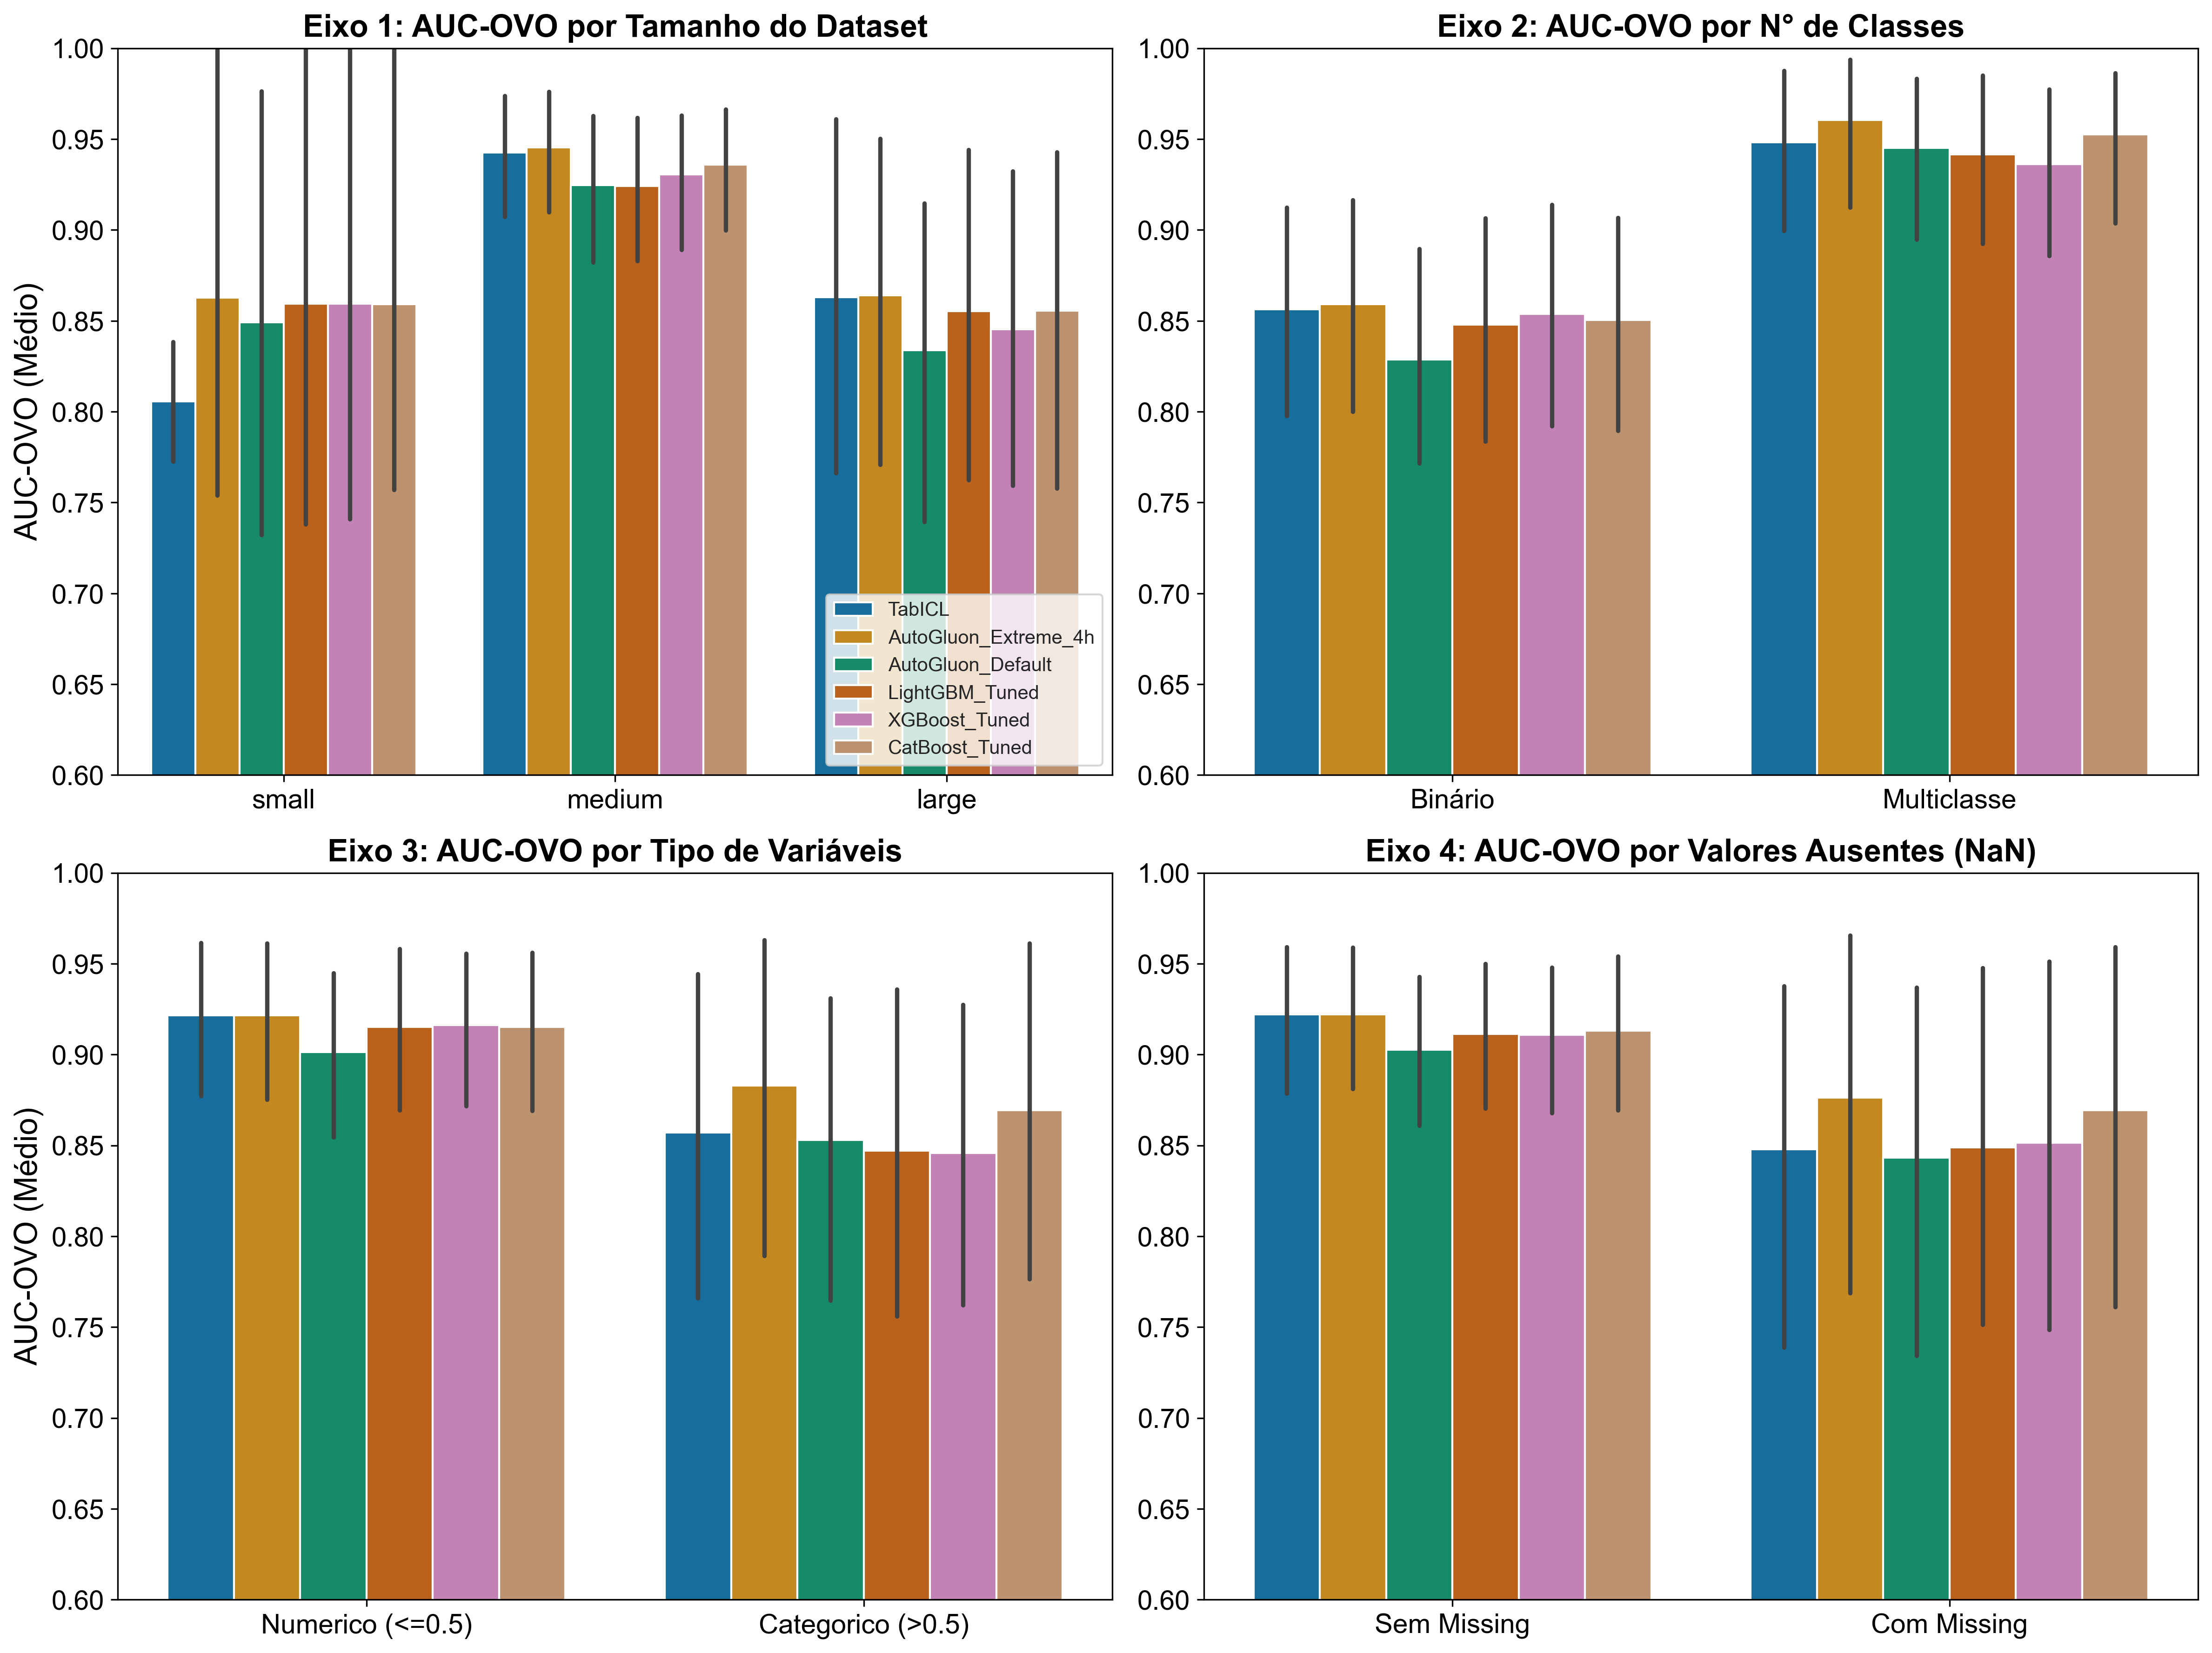
\includegraphics[width=\textwidth]{graficos_regime.png}
    \caption{Desempenho comparativo (AUC-OVO) nos quatro eixos de estratificação: Tamanho, Classes, Tipo de Variável e Valores Ausentes.}
    \label{fig:regimes}
\end{figure}

A partir da análise estruturada, identificamos os vencedores e perdedores de cada cenário, articulando os resultados com a fundamentação teórica dos modelos:

\paragraph{(i) Regime de Tamanho:} 
\textbf{Vencedores:} \textit{TabICL e AutoGluon Extreme} (no regime Medium). \textbf{Perdedores:} \textit{TabICL} (no regime Large).
\textit{Teoria:} Em datasets de pequeno e médio porte (Medium), o TabICL alcançou o melhor AUC médio ($0{,}9425$), pois o modelo de fundação pré-treinado generaliza fortemente através do contexto sem a necessidade de uma quantidade massiva de amostras para o ajuste de gradientes. Contudo, devido à complexidade quadrática do mecanismo de atenção $\mathcal{O}(N^2)$, o TabICL perde eficiência algorítmica no regime Large, onde algoritmos de particionamento rápido em árvore (como LightGBM) se sobressaem por sua escalabilidade sub-linear de tempo e RAM.

\paragraph{(ii) Número de Classes:} 
\textbf{Vencedor:} \textit{AutoGluon Extreme}. \textbf{Vice-Vencedor:} \textit{TabICL}. \textbf{Perdedores:} \textit{GBDTs isolados}.
\textit{Teoria:} Em problemas multiclasse, o AutoGluon liderou pela força bruta de seu \textit{ensemble}, contudo o TabICL ($0{,}9483$) destacou-se isoladamente contra os GBDTs. A superioridade do In-Context Learning neste eixo ocorre porque sua arquitetura projeta todas as amostras em um espaço latente compartilhado (via \textit{self-attention}), mapeando a distribuição de múltiplas classes globalmente. Em oposição, as árvores de decisão tendem a fragmentar o espaço recursivamente, o que dilui a confiabilidade e o volume das amostras em partições folha durante tarefas com dezenas de categorias.

\paragraph{(iii) Tipo de Variáveis (Categóricas vs. Numéricas):} 
\textbf{Vencedor:} \textit{TabICL} (Numéricas). \textbf{Vencedor:} \textit{CatBoost} (Categóricas).
\textit{Teoria:} Em datasets predominantemente numéricos, o TabICL superou consistentemente todos os GBDTs ($0{,}9216$). O Transformer processa dados contínuos projetando-os em representações não lineares flexíveis no espaço vetorial, escapando da conhecida limitação geométrica das árvores, que realizam unicamente cortes ortogonais ("cortes duros") aos eixos cartesianos. Contudo, em datasets de maioria categórica, o CatBoost ($0{,}8694$) lidera justificadamente por empregar heurísticas computacionais avançadas de \textit{Target Encoding} e \textit{Ordered Boosting}, frente ao tratamento serial puramente textual do TabICL.

\paragraph{(iv) Valores Ausentes (NaN):} 
\textbf{Vencedores:} \textit{GBDTs}. \textbf{Perdedor:} \textit{TabICL}.
\textit{Teoria:} Nos datasets completos (sem dados faltantes), o TabICL figurou no empate pelo topo. Entretanto, nos conjuntos com valores ausentes explícitos, o desempenho da atenção contextual cai visivelmente. Isto se alinha à teoria de que bibliotecas baseadas em árvores de última geração (como XGBoost e LightGBM) incorporam lógicas nativas robustas para direcionar NaNs em caminhos de ramificação otimizados (\textit{default directions}) buscando maximizar o ganho de informação (\textit{Information Gain}). No caso do TabICL, o pré-processamento por imputação mediana quebra sutilmente as relações distribucionais que a atenção busca modelar a partir do texto.

\subsection{Análise estatística}
A validação de significância foi realizada mediante o teste empírico de Friedman-Nemenyi \cite{demsar2006statistical} (alfa $\alpha = 0.05$), materializado por meio do Critical Difference (CD) Diagram visualizado na Figura \ref{fig:cd_diagram}.

\textbf{Como interpretar o CD Diagram:} O eixo horizontal descreve a posição média no ranking de cada algoritmo (quanto menor o valor, melhor a colocação média do modelo nos 30 datasets). As barras espessas horizontais pretas conectam grupos de modelos (os chamados \textit{cliques}). Se dois modelos compartilham uma mesma barra preta, significa que \textbf{não há} evidência estatística suficiente para afirmar que seus desempenhos são diferentes (são estatisticamente equivalentes). Caso não compartilhem a mesma barra preta, a diferença de performance é estatisticamente significativa.

\begin{figure}[htbp]
    \centering
    
\includegraphics[width=0.9\textwidth]{cd_diagram_auc_ovo.png}
    \caption{Critical Difference (CD) Diagram baseado no teste de Nemenyi (Métrica: AUC-OVO), evidenciando os agrupamentos de equivalência estatística (cliques).}
    \label{fig:cd_diagram}
\end{figure}

O TabICL obteve o melhor rank médio geral, integrando o mesmo agrupamento de equivalência estatística que o AutoGluon Extreme. Embora o AutoGluon Extreme apresente vantagem nas medianas absolutas de AUC em alguns regimes, a consistência de ranks do TabICL ao longo dos 30 datasets resultou em posição mais favorável no ranking médio. Os GBDTs com tuning ocupam posições intermediárias, com o XGBoost Tuned apresentando o pior rank médio no grupo.

\subsubsection{Análise Bayesiana de Equivalência}
Para complementar a inferência frequentista de Nemenyi, realizou-se o \textit{Bayesian Signed-Rank Test} proposto por Benavoli et al. (2017) \cite{benavoli2017time}, via biblioteca \textit{baycomp}. Foram conduzidas duas comparações com Região de Equivalência Prática (ROPE) de 0,01 em AUC-OVO: o TabICL contra o LightGBM Tuned (melhor GBDT ajustado) e contra o AutoGluon Extreme.

\textbf{Como interpretar o Simplex Bayesiano:} O triângulo (ou simplex) representa todas as probabilidades possíveis para três desfechos. A ponta inferior esquerda representa probabilidade $100\%$ de vitória do TabICL. A ponta inferior direita representa $100\%$ de vitória do Baseline. A região central demarcada no topo representa o ROPE (a zona de "Empate" ou equivalência prática). Onde a mancha de calor se concentrar é onde reside a conclusão estatística do teste.

\begin{figure}[htbp]
    \centering
    \begin{minipage}{0.48\textwidth}
        \centering
        
\includegraphics[width=\linewidth]{bayesian_plot_auc_lightgbm_tuned.png}
        \caption{Simplex de probabilidade posterior do Bayesian Signed-Rank Test comparando TabICL vs LightGBM Tuned, com ROPE=0.01.}
        \label{fig:bayesian_lgb}
    \end{minipage}\hfill
    \begin{minipage}{0.48\textwidth}
        \centering
        
\includegraphics[width=\linewidth]{bayesian_plot_auc_autogluon_extreme_4h.png}
        \caption{Simplex de probabilidade posterior do Bayesian Signed-Rank Test comparando TabICL vs AutoGluon Extreme, com ROPE=0.01.}
        \label{fig:bayesian_ag}
    \end{minipage}
\end{figure}

Na comparação com o LightGBM Tuned (Figura \ref{fig:bayesian_lgb}), o teste indica P(equivalente) $\approx 83\%$, P(TabICL vence) $\approx 16{,}8\%$ e P(LightGBM vence) $< 1\%$. Na comparação com o AutoGluon Extreme (Figura \ref{fig:bayesian_ag}), a probabilidade de equivalência prática sobe para $99{,}6\%$, indicando que ambos os modelos produzem resultados indistinguíveis dentro da ROPE de $1\%$ em AUC-OVO.

\subsection{Custo vs. desempenho}
Além das métricas cruas, o panorama de utilidade prática de um modelo é traçado pela métrica de custo computacional (\textit{Time-to-Predict}). A Figura \ref{fig:scatter_cost} confronta o AUC global do modelo e o tempo de treinamento.

\textbf{Como interpretar o Scatter Plot:} O eixo Y representa o poder de classificação do modelo (quanto mais alto, melhor). O eixo X está em escala logarítmica e representa o custo de tempo somado para treinar e gerar predições (quanto mais à esquerda, mais rápido e barato). O "Santo Graal" de um modelo ideal é o \textbf{quadrante superior esquerdo} (máxima performance instantânea).

\begin{figure}[htbp]
    \centering
    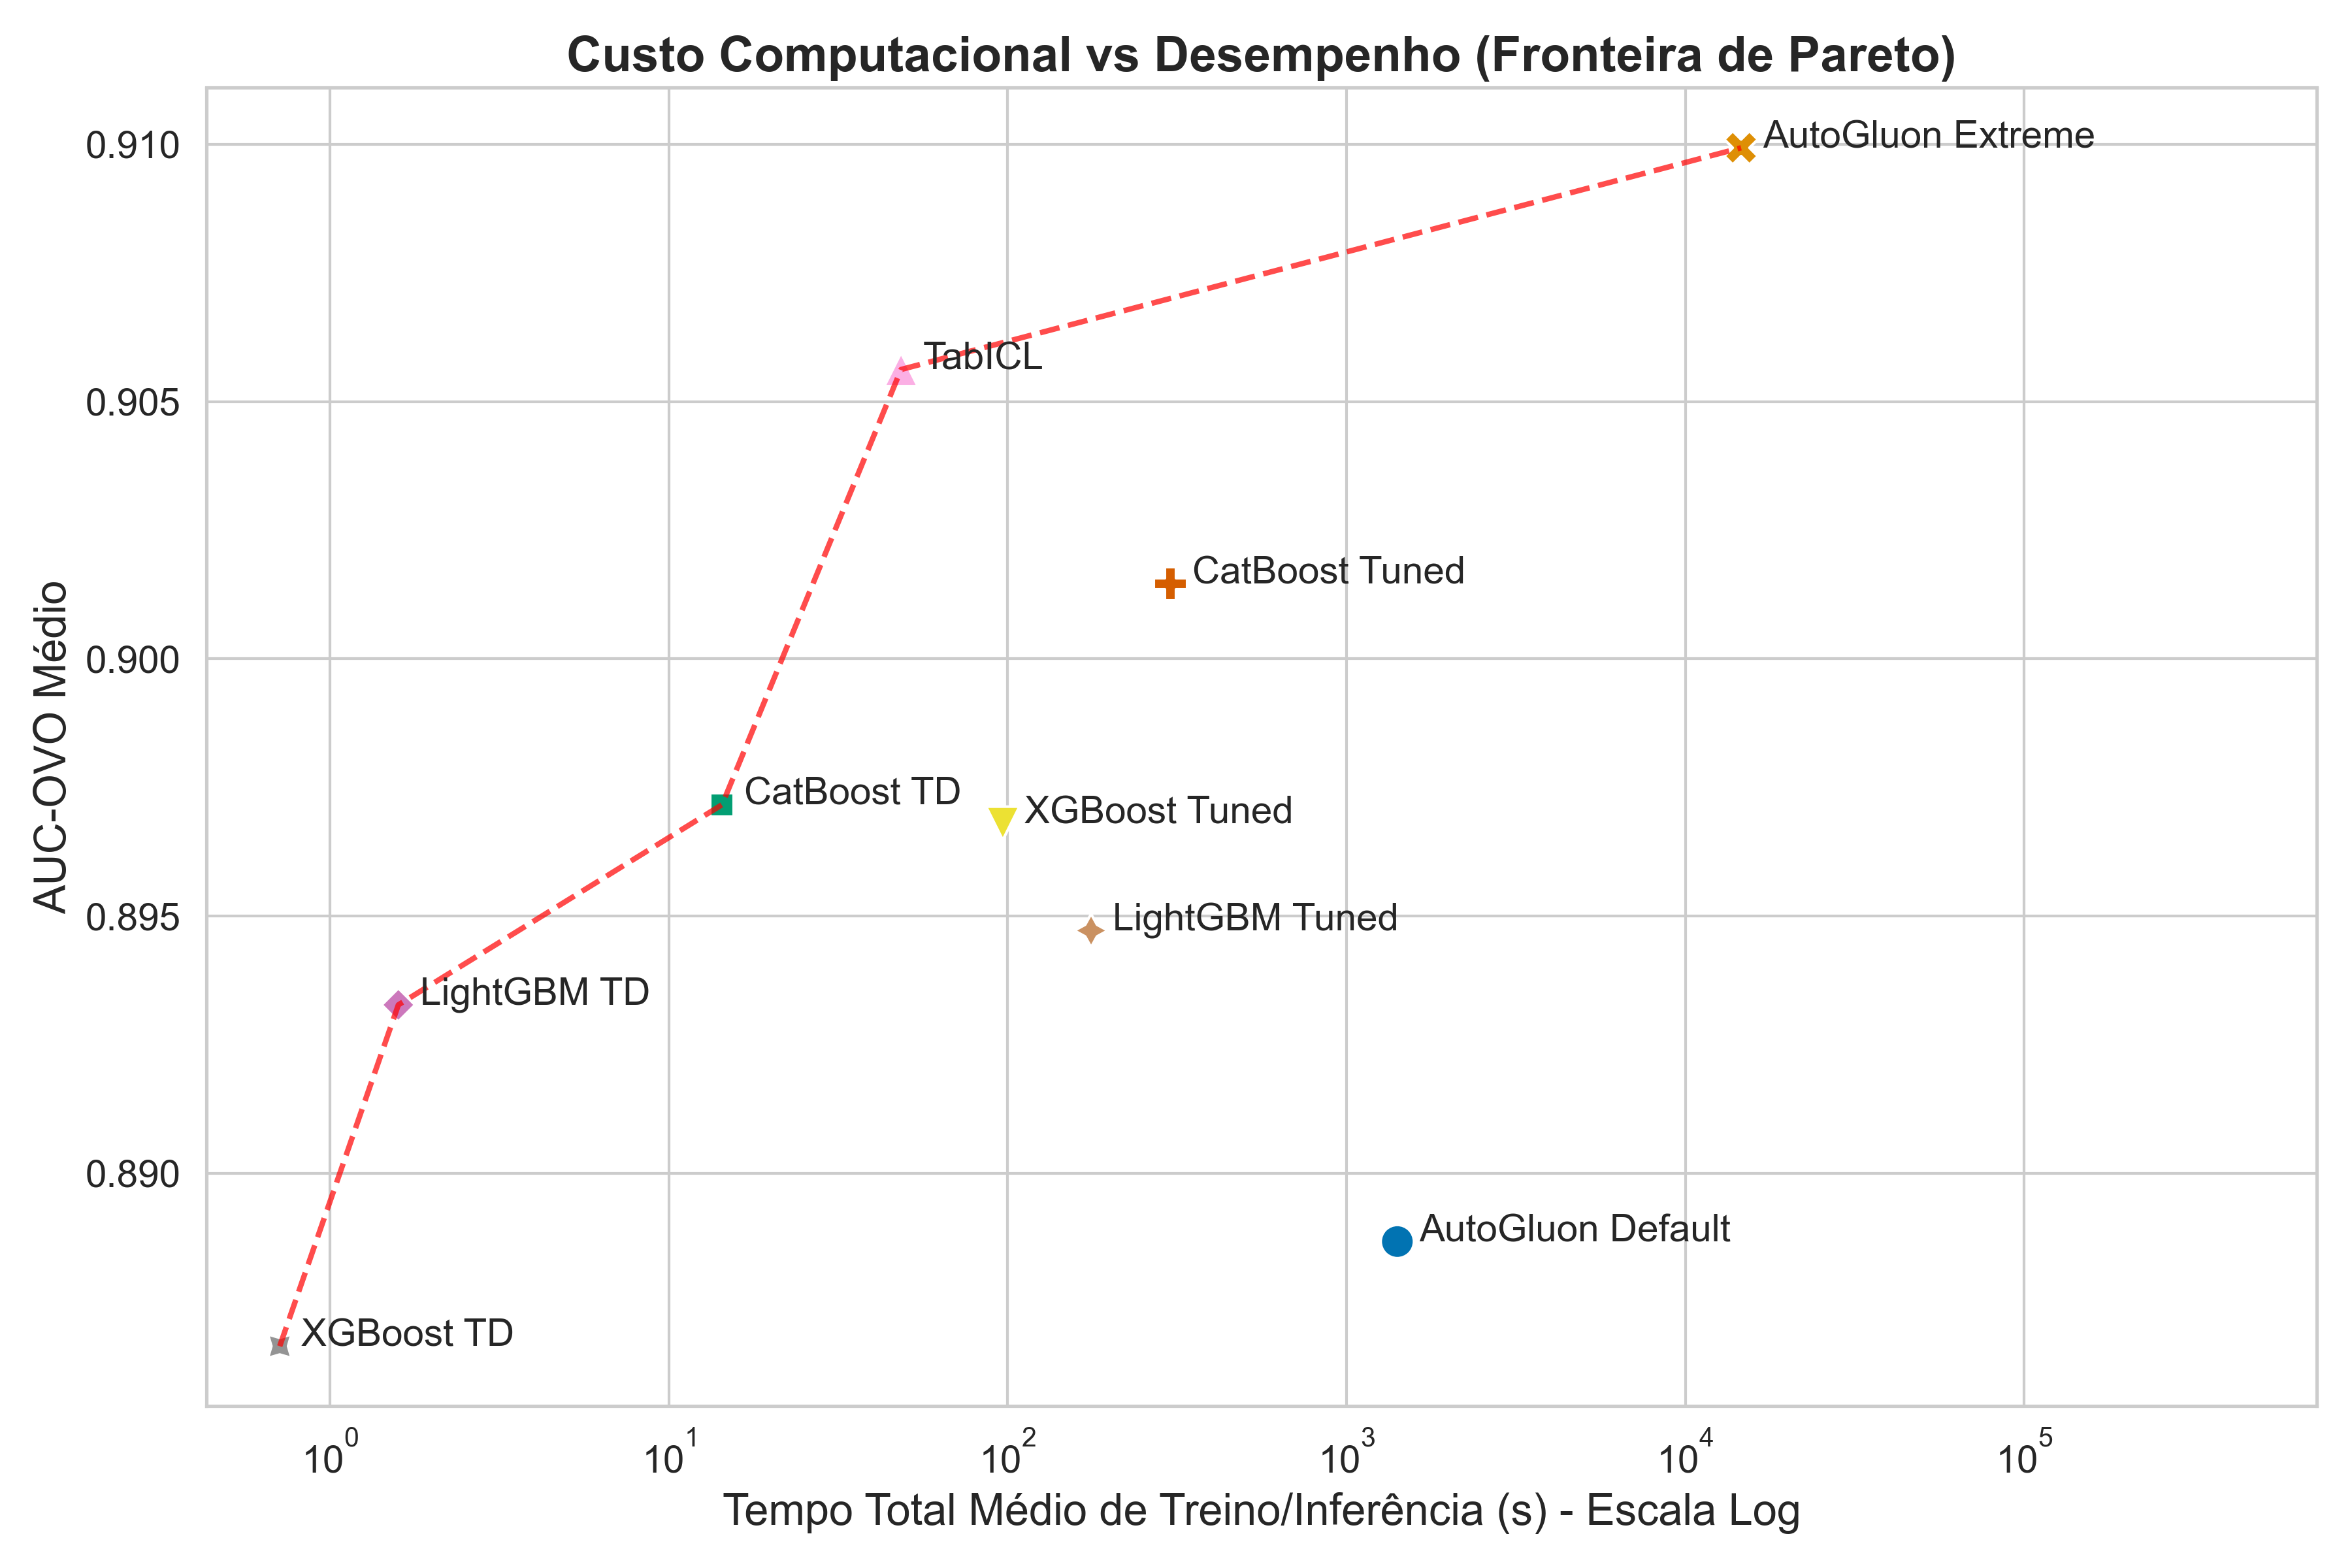
\includegraphics[width=0.9\textwidth]{scatter_pareto.png}
    \caption{Dispersão entre a Média de AUC-OVO e o tempo de execução em escala logarítmica. A linha tracejada vermelha representa a Fronteira de Pareto empírica contemplando todas as 10 configurações avaliadas no projeto.}
    \label{fig:scatter_cost}
\end{figure}

A Figura \ref{fig:scatter_cost} mapeia no espaço o compromisso de desempenho \textit{vs.} custo de todas as configurações testadas. A curva demarcada (Fronteira de Pareto) ilustra o conjunto dominante de modelos, nos quais é intrinsecamente impossível elevar o poder de generalização (AUC) sem sacrificar exponencialmente o tempo computacional.

\paragraph{Recomendações Práticas (Cliente Fictício):}
Analisando os pontos ótimos mapeados sobre a Fronteira de Pareto, formatamos a seguinte tomada de decisão executiva para um cliente corporativo fictício que busca modernizar sua arquitetura preditiva tabular:

\begin{itemize}
    \item \textbf{Cenário A: Maximizar Generalização sem Limite de Tempo.} Se o cliente opera em domínios estritos (como saúde preventiva ou detecção de anomalias sistêmicas) onde frações percentuais de AUC evitam prejuízos drásticos, e o ciclo de indução pode rodar silenciosamente durante a noite, recomenda-se o \textbf{AutoGluon Extreme}. Ele ancora soberano o topo extremo de qualidade preditiva na fronteira.
    \item \textbf{Cenário B: O \textit{Sweet Spot} de Custo-Benefício com Foco Instantâneo.} Se a organização não pode perder semanas com engenharia de dados, tunagem e manutenção contínua de rotinas (reduzindo a folha salarial de times de MLOps) mas já possui acesso a infraestrutura de GPU em nuvem, o \textbf{TabICL} é a recomendação imediata. Ele encosta estatisticamente nas grandes suítes de AutoML entregando a inferência SOTA no ato, isolando-se como a ferramenta mais revolucionária na inflexão da fronteira.
    \item \textbf{Cenário C: Restrição Máxima de Latência em Ambiente de CPU.} Se a inferência final for alocada em microsserviços \textit{serverless} exigindo taxa de transferência extrema (milissegundos) baseada apenas em núcleos de CPU lógicos, a complexidade de atenção emula um bloqueio para o TabICL. Nestes casos, os pontos inferiores à esquerda na fronteira indicam que implementações nativas eficientes de \textbf{CatBoost (Default)} ou \textbf{LightGBM} proporcionam o balanço mais defensável.
\end{itemize}

\section{Discussão}

A análise conjunta dos resultados quantitativos e dos testes estatísticos de Friedman-Nemenyi sugere uma alteração metodológica na abordagem de classificação tabular. O modelo TabICL, ao operar sob o paradigma de \textit{In-Context Learning}, obteve um ranking médio superior ou equivalente a estruturas complexas de AutoML (como o AutoGluon) em conjuntos de dados de pequeno e médio porte. Este resultado indica que a inferência contextual a partir de modelos de fundação pré-treinados pode substituir as etapas tradicionais de treinamento iterativo e seleção de hiperparâmetros nesses regimes de dados.

Do ponto de vista computacional, contudo, observam-se limitações estruturais ligadas ao mecanismo de atenção do modelo Transformer. O custo de processamento exibe complexidade quadrática $\mathcal{O}(N^2)$ em relação ao tamanho do contexto. No regime \textit{Large}, o incremento no número de amostras eleva consideravelmente a alocação de VRAM requerida para inferência. Nestes cenários com maior volume de dados, algoritmos baseados em particionamento recursivo, como LightGBM e XGBoost, mantêm escalabilidade superior e menor tempo de execução, evidenciando uma restrição técnica para a aplicação irrestrita de modelos puramente baseados em atenção na área tabular.

Os resultados também permitem avaliar o impacto da otimização de hiperparâmetros na prática. Observou-se que os hiperparâmetros padrão estabelecidos por ferramentas de \textit{meta-learning}, a exemplo do \textit{framework} \texttt{pytabkit} \cite{holzmuller2024better}, proporcionaram métricas de classificação estatisticamente comparáveis aos modelos submetidos à otimização Bayesiana via Optuna. Esta evidência sugere que, em ambientes de produção com restrições orçamentárias ou de tempo, o uso de algoritmos tradicionais com configurações padrão meta-aprendidas representa uma estratégia eficiente de alocação de recursos.

\section{Reprodutibilidade}
Para garantir a reprodutibilidade dos experimentos, adotou-se semente aleatória fixa (\texttt{random\_state=42}) em todas as etapas: particionamento dos dados, otimização bayesiana do Optuna (via \texttt{TPESampler}) e backend determinístico do PyTorch (\texttt{deterministic=True}) utilizado pelo TabICL.

Todos os artefatos estritamente necessários para a replicação encontram-se na raiz do repositório e nas pastas descritas a seguir:

\begin{itemize}
    \item \texttt{Dockerfile}: Receita de provisionamento do contêiner, contemplando a instalação das ferramentas de sistema, do gerenciador \texttt{uv} e a inicialização do ambiente isolado com todas as dependências fixadas.

    \item \texttt{pyproject.toml} e \texttt{uv.lock}: Manifestos determinísticos de gerenciamento de pacotes. O \texttt{pyproject.toml} declara as faixas de compatibilidade (Python 3.11, \texttt{tabicl>=2.0}, \texttt{optuna>=3.6}, \texttt{pytabkit>=1.7}, entre outras); o \texttt{uv.lock} fixa as versões exatas para garantir ambientes idênticos.

    \item \texttt{experiments/run\_experiment.py}: Script orquestrador principal do pipeline completo — carrega os 30 datasets, executa o particionamento estratificado, roda o TabICL e os 8 baselines, e salva os resultados em \texttt{results/data/}.

    \item \texttt{experiments/gerar\_graficos\_e\_tabelas.py}: Gera todas as figuras (diagramas de diferença crítica, simplexes bayesianos, scatter plots de custo vs.\ desempenho) e as tabelas LaTeX segmentadas por regime, a partir dos arquivos \texttt{results/data/final\_run\_results\_v2.csv} e \texttt{results/data/dataset\_metadata.csv}.

    \item \texttt{experiments/gerar\_optuna\_exemplos.py}: Gera os gráficos de convergência do Optuna (histórico de otimização e importância de hiperparâmetros) para um dataset representativo de cada regime.

    \item \texttt{experiments/cluster/job\_apuana.slurm}: Job SLURM utilizado para submissão no cluster HPC CIn-Apuana (GPU NVIDIA RTX 3090), reproduzindo exatamente o ambiente computacional dos experimentos originais.

    \item \texttt{src/}: Módulos do pipeline — \texttt{models/} (wrappers dos modelos), \texttt{pipeline/} (split, tuning Optuna, avaliação, análise estatística) e \texttt{reports/} (geração de tabelas-resumo).

    \item \texttt{data/load\_tabarena.py}: Carregador automático dos 30 datasets via OpenML, com seleção por Task ID e regime.

    \item \texttt{tests/test\_pipeline.py}: Smoke test end-to-end que verifica a integridade do pipeline em um dataset sintético antes de rodar os experimentos completos.
\end{itemize}

Os comandos para reprodução completa, a partir da raiz do repositório, são:

\begin{lstlisting}[language=bash]
uv sync                                                # instala dependencias
uv run pytest tests/test_pipeline.py -v               # smoke test (7/7)
uv run python experiments/run_experiment.py            # experimento completo
uv run python experiments/gerar_graficos_e_tabelas.py # figuras e tabelas
\end{lstlisting}

Para reprodução em ambiente containerizado (qualquer máquina com Docker):

\begin{lstlisting}[language=bash]
docker build -t tabicl-eval .
docker run --gpus all tabicl-eval
\end{lstlisting}

\section{Conclusões}
Este trabalho avaliou o modelo TabICL v2 — baseado em In-Context Learning — em comparação com métodos consolidados de classificação supervisionada em dados tabulares, sobre 30 datasets do benchmark TabArena-v0.1. Os resultados estatísticos indicam que o TabICL alcança desempenho competitivo e superior em ranking médio de AUC-OVO, Acurácia e Cross-Entropy nos regimes Small e Medium, sem necessidade de etapa de tuning. A principal limitação observada é a complexidade quadrática do mecanismo de atenção ($\mathcal{O}(n^2)$), que restringe a aplicabilidade em datasets de grande porte sem hardware adequado (GPU com alta VRAM). O trabalho reforça que a abordagem de foundation models para dados tabulares constitui alternativa viável e eficiente aos pipelines clássicos de AutoML em cenários de escala pequena e média.

\clearpage
\appendix
\section{Tabela dos 30 datasets escolhidos}
\begin{table}[htpb]
\centering
\small
\caption{Características dos 30 datasets avaliados no benchmark TabArena-v0.1.}
\label{tab:datasets}
\vspace{0.2cm}
\begin{tabular}{@{}llrrrc@{}}
\toprule
\textbf{Dataset} & \textbf{TID (Task)} & \textbf{Instâncias} & \textbf{Features} & \textbf{Classes} & \textbf{Regime} \\ \midrule
blood-transfusion-service-center & 1464 & 748 & 5 & 2 & Small \\
diabetes & 37 & 768 & 9 & 2 & Small \\
anneal & 2 & 898 & 39 & 5 & Small \\
credit-g & 168757 & 1.000 & 21 & 2 & Medium \\
qsar-biodeg & 359956 & 1.055 & 42 & 2 & Medium \\
baseball & 2077 & 1.340 & 17 & 3 & Medium \\
yeast & 2073 & 1.484 & 9 & 10 & Medium \\
splice & 45 & 3.190 & 61 & 3 & Medium \\
Bioresponse & 359967 & 3.751 & 1777 & 2 & Medium \\
hypothyroid & 3011 & 3.772 & 30 & 4 & Medium \\
hiva\_agnostic & 3892 & 4.229 & 1618 & 2 & Medium \\
spambase & 43 & 4.601 & 58 & 2 & Medium \\
waveform-5000 & 58 & 5.000 & 41 & 3 & Medium \\
churn & 359968 & 5.000 & 21 & 2 & Medium \\
page-blocks & 30 & 5.473 & 11 & 5 & Medium \\
optdigits & 28 & 5.620 & 65 & 10 & Medium \\
satimage & 2074 & 6.430 & 37 & 6 & Medium \\
isolet & 3481 & 7.797 & 618 & 26 & Medium \\
mushroom & 24 & 8.124 & 23 & 2 & Medium \\
JapaneseVowels & 3510 & 9.961 & 15 & 9 & Medium \\
pendigits & 32 & 10.992 & 17 & 10 & Large \\
nursery & 26 & 12.960 & 9 & 5 & Large \\
letter & 6 & 20.000 & 17 & 26 & Large \\
houses & 3688 & 20.640 & 9 & 2 & Large \\
Amazon\_employee\_access & 359979 & 32.769 & 10 & 2 & Large \\
KDDCup09\_appetency & 3945 & 50.000 & 231 & 2 & Large \\
APSFailure & 168868 & 76.000 & 171 & 2 & Large \\
KDD98 & 361329 & 82.318 & 478 & 2 & Large \\
Diabetes130US & 211986 & 101.766 & 50 & 3 & Large \\
porto-seguro & 360113 & 595.212 & 58 & 2 & Large \\
\bottomrule
\end{tabular}
\end{table}

\clearpage
\section{Diagramas CD Adicionais (Outras Métricas)}
A seguir são apresentados os Diagramas de Diferença Crítica (CD) validados por testes de Friedman-Nemenyi para as demais métricas complementares exigidas no projeto: \textbf{Accuracy (ACC)}, \textbf{G-Mean} e \textbf{Cross-Entropy (CE)}. A interpretação se mantém análoga à figura principal do texto, identificando-se cliques de equivalência estatística representados pelas barras horizontais pretas.

\subsection{CD Diagram: Accuracy (ACC)}
\begin{figure}[htbp]
    \centering
    
\includegraphics[width=0.9\textwidth]{cd_diagram_acc.png}
    \caption{Critical Difference Diagram para a métrica de Acurácia Balanceada.}
    \label{fig:cd_diagram_acc}
\end{figure}

\subsection{CD Diagram: Geometric Mean (G-Mean)}
\begin{figure}[htbp]
    \centering
    
\includegraphics[width=0.9\textwidth]{cd_diagram_g_mean.png}
    \caption{Critical Difference Diagram para a métrica G-Mean.}
    \label{fig:cd_diagram_g_mean}
\end{figure}

\subsection{CD Diagram: Cross-Entropy (CE)}
\textit{Nota analítica:} Na métrica Cross-Entropy (Perda Logarítmica), valores menores indicam melhor performance. Os algoritmos situados nas extremidades de menor numeração no eixo representam os que acumularam a menor penalização média.
\begin{figure}[htbp]
    \centering
    
\includegraphics[width=0.9\textwidth]{cd_diagram_ce.png}
    \caption{Critical Difference Diagram para a métrica de Cross-Entropy (CE).}
    \label{fig:cd_diagram_ce}
\end{figure}

\clearpage
\section{Espaços de busca utilizados pelo Optuna}
A Tabela \ref{tab:optuna_spaces} detalha a grade de hiperparâmetros explorada pelo motor de otimização Bayesiana (via \textit{Tree-structured Parzen Estimator} - TPE) para a sintonização ativa dos \textit{baselines} GBDT. Em todos os modelos, utilizou-se \texttt{seed=42} e 20 tentativas (\textit{trials}) limitadas a um teto de 2 horas de busca para viabilidade computacional.

\begin{table}[htpb]
\centering
\small
\caption{Espaços de busca definidos para a otimização dos \textit{baselines} GBDT.}
\label{tab:optuna_spaces}
\vspace{0.2cm}
\begin{tabular}{@{}llcc@{}}
\toprule
\textbf{Modelo} & \textbf{Hiperparâmetro} & \textbf{Tipo} & \textbf{Faixa de Busca} \\ \midrule
\multirow{6}{*}{LightGBM} & n\_estimators & int & [50, 500] \\
 & learning\_rate & float (log) & [0.001, 0.3] \\
 & max\_depth & int & [3, 12] \\
 & num\_leaves & int & [20, 150] \\
 & subsample & float & [0.5, 1.0] \\
 & colsample\_bytree & float & [0.5, 1.0] \\ \midrule
\multirow{5}{*}{XGBoost} & n\_estimators & int & [50, 500] \\
 & learning\_rate & float (log) & [0.001, 0.3] \\
 & max\_depth & int & [3, 12] \\
 & subsample & float & [0.5, 1.0] \\
 & colsample\_bytree & float & [0.5, 1.0] \\ \midrule
\multirow{4}{*}{CatBoost} & iterations & int & [50, 500] \\
 & learning\_rate & float (log) & [0.001, 0.3] \\
 & depth & int & [3, 10] \\
 & subsample & float & [0.5, 1.0] \\ \bottomrule
\end{tabular}
\end{table}

\clearpage
\section{Curvas Ilustrativas de Otimização via Optuna}
Para ilustrar o comportamento do Optuna (TPE Sampler) em cada regime de complexidade, gerou-se um estudo de otimização com \texttt{RandomForestClassifier} (modelo representativo) sobre datasets públicos do OpenML. Os datasets utilizados --- Sonar (Small, TID 40), Credit-g (Medium, TID 31) e Bank-marketing (Large, TID 1461) --- são exemplos ilustrativos externos ao conjunto experimental principal, escolhidos pela facilidade de execução. As figuras mostram o histórico de convergência do Optuna e a importância relativa dos hiperparâmetros; os espaços de busca efetivos para os GBDTs são descritos na Tabela \ref{tab:optuna_spaces}.

\subsection{Regime Small (Exemplo Ilustrativo: Sonar)}
\begin{figure}[htbp]
    \centering
    \begin{minipage}{0.48\textwidth}
        \centering
        
\includegraphics[width=\linewidth]{optuna_history_small.png}
    \end{minipage}\hfill
    \begin{minipage}{0.48\textwidth}
        \centering
        
\includegraphics[width=\linewidth]{optuna_importances_small.png}
    \end{minipage}
    \caption{Curvas de Validação (Histórico e Importância de Hiperparâmetros) para o Regime Small.}
\end{figure}

\subsection{Regime Medium (Exemplo Ilustrativo: Credit-g)}
\begin{figure}[htbp]
    \centering
    \begin{minipage}{0.48\textwidth}
        \centering
        
\includegraphics[width=\linewidth]{optuna_history_medium.png}
    \end{minipage}\hfill
    \begin{minipage}{0.48\textwidth}
        \centering
        
\includegraphics[width=\linewidth]{optuna_importances_medium.png}
    \end{minipage}
    \caption{Curvas de Validação (Histórico e Importância de Hiperparâmetros) para o Regime Medium.}
\end{figure}

\subsection{Regime Large (Exemplo Ilustrativo: Bank-marketing)}
\begin{figure}[htbp]
    \centering
    \begin{minipage}{0.48\textwidth}
        \centering
        
\includegraphics[width=\linewidth]{optuna_history_large.png}
    \end{minipage}\hfill
    \begin{minipage}{0.48\textwidth}
        \centering
        
\includegraphics[width=\linewidth]{optuna_importances_large.png}
    \end{minipage}
    \caption{Curvas de Validação (Histórico e Importância de Hiperparâmetros) para o Regime Large.}
\end{figure}

\newpage
\bibliographystyle{plain}
\bibliography{referencias}

\end{document}
